\chapter{MITRE Caldera}
MITRE nasce come organizzazione no-profit nel 1958, per offrire consulenza sull'ingegneria di sistema ad agenzie governative sia civili sia militari.\\
Negli anni, si è distinta tra le strutture aziendali grazie al suo impatto in aree quali ingegneria aerospaziale, cybersecurity ed intelligenza artificiale; sviluppando tools utili ed implementati da molte attuali agenzie. Uno tra questi è \textsc{MITRE ATT\&CK}.\\
Pubblicata per la prima volta nel 2013, è globalmente accessibile a tutti e rappresenta una linea guida sulle conoscenza base di tattiche, tecniche e procedure di avversari basati su osservazioni reali. In poche parole, funge da modello nello sviluppo di minacce e metodologie nel settore della cyber sicurezza.\\
\begin{figure}[h!]
    \centering
    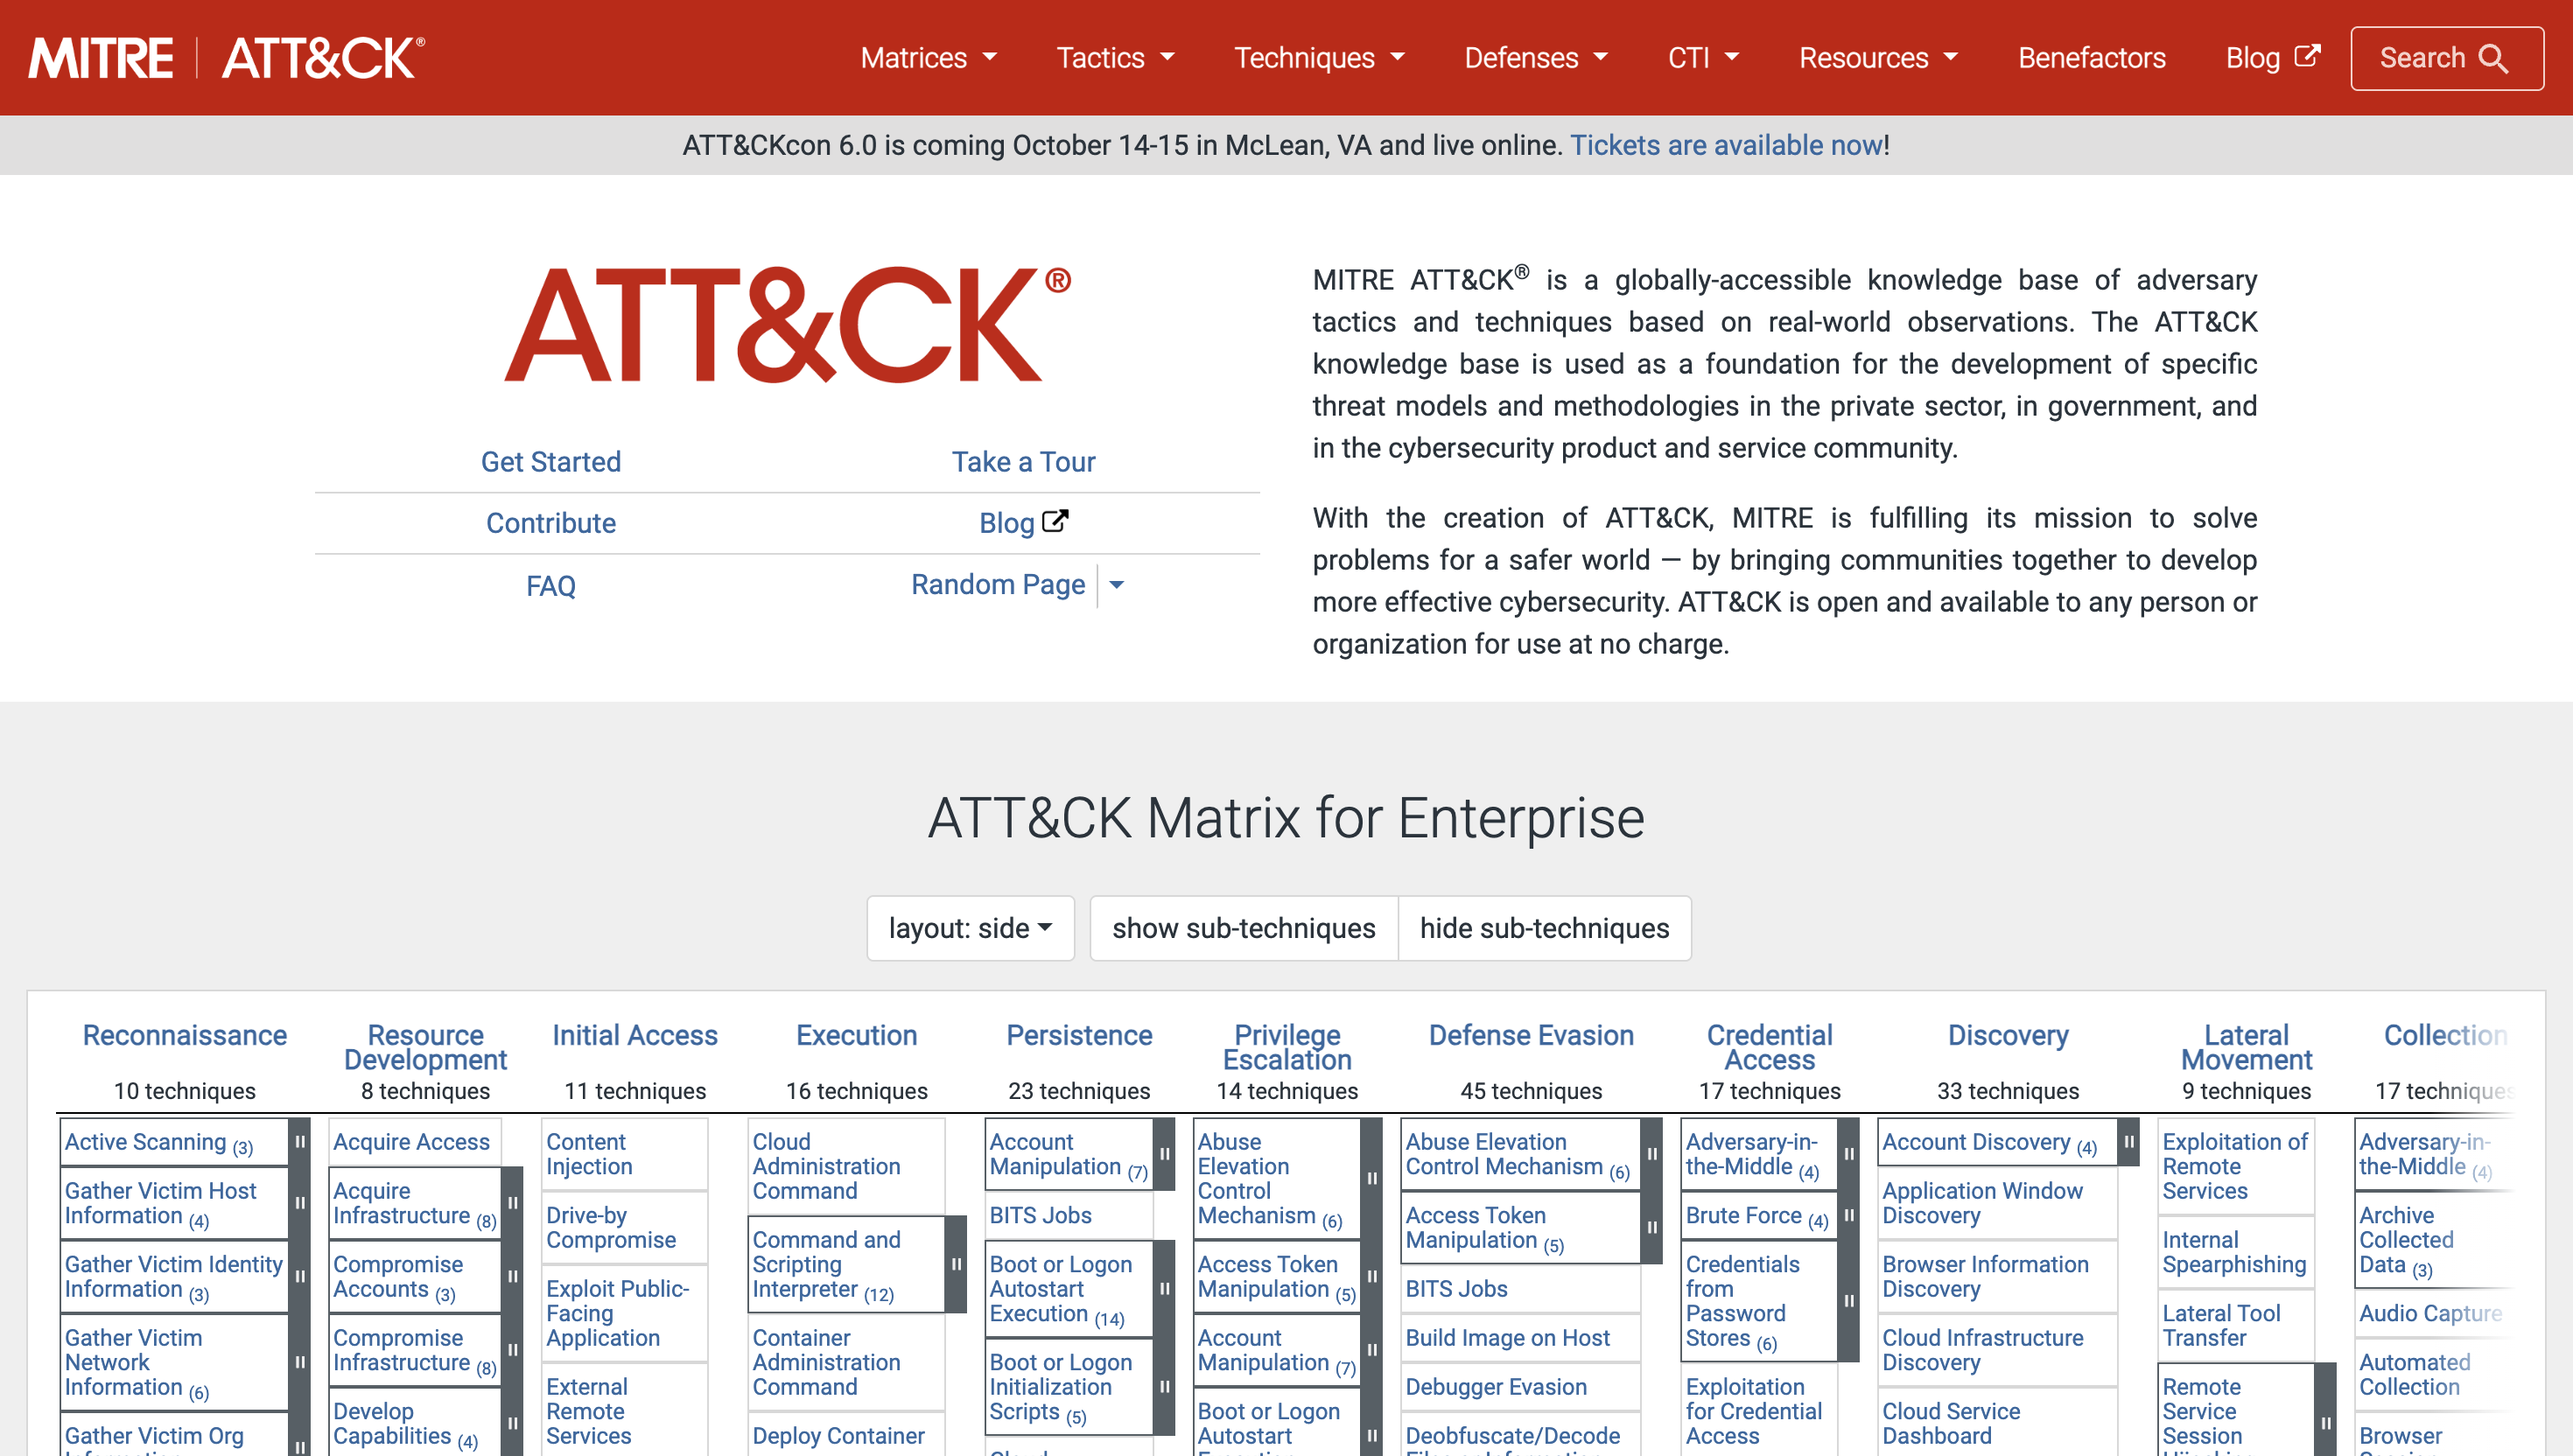
\includegraphics[width=0.7\linewidth]{images/MITRE_ATT&CK.png}
    \caption{Homepage di MITRE ATT\&CK}
\end{figure}\\
Il modello focalizza l'attenzione su come un attaccante interagisce con il sistema target durante un'operazione di breach, descrivendo i vari step partendo da un vettore di attacco e descrivendo i mezzi utilizzati.\\
Sulla base di questi concetti e descrizioni, è stato rilasciato nel 2017 uno strumento capace di emulare e, soprattutto, automatizzare il comportamento di un malintenzionato all'interno della rete, permettendo al team di difesa (Blue team) di concentrarsi su aspetti più specifici e nello stesso tempo facilità la progettazione della kill chain al team di attacco (Red Team): si tratta di Caldera\textsuperscript{TM} (Cyber Adversary Language and Decision Engine for Red Team Automation) ed è l'attore principale del progetto.
\newpage

\section{Componenti \& funzionalità\label{cald}}
    \begin{wrapfigure}{r}{0.2\textwidth}
        \vspace{-10pt}
        \centering
        
\includegraphics[width=0.2\textwidth]{images/Caldera_post_icon.png}
        \caption{Logo Caldera}
    \end{wrapfigure}
    Caldera nasce come web agent funzionante principalmente in Google Chrome; l'ultima versione rilasciata attualmente è la v5.3.0 e lo sviluppo continuo ha portato ad un'interfaccia molto user-friendly; sono state anche aggiunte diverse funzionalità in modo da rendere l'esperienza molto più interattiva e coinvolgente per gli utenti di Caldera.
    Il tool è costruito su due semplici componenti:
    \begin{itemize}
        \item \textbf{Core system:} Il codice sorgente del framework, include un server di Command-and-Control (C2) con una REST API ed un'interfaccia web in modo da avere pieno controllo dell'agente una volta inserito.
        \item \textbf{Plugins:} Repositories esterne, che dipendono dal core system, offrono funzionalità aggiuntive rispetto a quelle di default di Caldera.
    \end{itemize}
    Caldera sfrutta il framework ATT\&CK per identificare e riprodurre il comportamento di veri attaccanti registrati nel corso degli anni, costruendo un profilo che rispecchia in modo preciso una possibile minaccia reale ed attuale. È inclusa la possibilità di utilizzare il tool per delle diagnosi e delle ricerche dal lato Blue Team ma, non essendo lo scope di questo laboratorio, saranno esplorati solo le feature riguardanti l'automazione di ingaggi Red Team. L'architettura è centralizzata; è basata su un costrutto server-client in cui il secondo è rappresentato dall'agente installato all'interno dell'host da compromettere, mentre il server amministra le operazioni e rende disponibili all'utente tutte le informazioni ricavate dai vari agent. Fondamentalmente, dopo aver pianificato le azioni da seguire, il server attende la connessione da parte dei client e, successivamente, avvia le singole operazioni, anche attraverso host intermedi a seguito di movimenti laterali. Il linguaggio di programmazione principe del framework è Python.\\
    Di seguito, una lista dei concetti principali che si incrociano andando ad utilizzare il software di adversary emulation:
    \begin{itemize}
        \item \textbf{Agent \& groups:} Rappresentano programmi software, i quali si collegano a Caldera ad intervalli regolari in modo da ricevere istruzioni.\\
        Attualmente, sono già presenti un certo numero di agenti predefiniti che presentano diverse e singole funzionalità.
        \begin{enumerate}
            \item \textit{Sandcat:} Un agente implementato in Golang che permette di comunicare tramite canali C2 come HTTP, DNS tunneling o Github GIST.
            \item \textit{Manx:} Sempre implementato tramite Golang, ma comunica grazie a un contatto TCP e funziona come una reverse-shell.
            \item \textit{Ragdoll:} Costruito con Python, utilizza HTML per creare un contatto. 
        \end{enumerate}
        Un insieme di agenti può costituire un gruppo e sono spesso usati durante le operazioni di Red Team, perché determinano su che agenti eseguire le \textit{abilities} e, soprattutto, aggiungono del parallelismo nelle varie fasi. Tenendo conto della possibilità di avere degli agenti Blue Team, la presenza di gruppi divisi permette un'organizzazione più efficiente ed un'analisi approfondita su attacchi e difese automatizzati.
        \item \textbf{Abilities \& adversaries:} Quando parliamo di \textit{ability}, ci riferiamo a una specifica tattica o tecnica implementata in ATT\&CK che può essere eseguita da agenti in funzione. In particolare, sono inclusi: i comandi da eseguire, le piattaforme in cui eseguirlo (es. Windows Powershell), i payload da allegare ed un'impostazione per il formato dell'output da far arrivare al server.\\
        Un gruppo di \textit{abilities} costituiscono il profilo di un determinato avversario. Molti di essi sono già presenti nell'implementazione predefinita di Caldera e permettono di determinare che \textit{abilities} saranno eseguite in un'ipotetica operazione. Nonostante ciò, l'utente ha libera scelta sulla modifica del profilo avversario; è possibile addirittura crearne uno personalizzato con relative \textit{abilities} atomiche.
        \item \textbf{Operations:} Per avviare un'operazione, bisogna aver già installato un agent funzionante e selezionare il profilo della minaccia da eseguire. È possibile lanciare diverse operazioni in parallelo ed ogni agente può essere incluso in varie di queste.\\
        Durante i singoli piani di attacco, entrano in gioco dei moduli in grado di garantire il buon esito dell'operazione.
        \begin{enumerate}
            \item \textit{Planner:} Si occupa della configurazione delle modalità secondo cui vengono eseguite le \textit{abilities}. Sono disponibili di default diversi esempi di tipi di planner: atomic, esegue le singole \textit{abilities} in base al profilo dell'avversario; batch, esegue tutte le \textit{abilities} in una volta; infine, buckets, esegue le \textit{abilities} raggruppate in base alla tattica ATT\&CK.
            \item \textit{Facts:} Pezzi d'informazione riguardanti un dato sistema host e correlati con l'attributo \texttt{Command} nelle \textit{abilities}, tra i suoi elementi abbiamo la proprietà, il valore e lo score.\\
            Una volta inviata l'\textit{ability}, il server individua eventuali variabili e controlla quali di questi possono essere sostituiti con i facts a disposizione.
            \item \textit{Parser:} Utilizzato da Caldera per aggiungere ogni fact collezionato all'operazione. Si analizza l'output di un'\textit{ability} per estrarre potenziali info da utilizzare per i link futuri, tutto questo configurabile grazie a delle regole sui \textit{facts}.
            \item \textit{Link:} Generato per ogni agente durante l'esecuzione di un'ability. Se tutti i requisiti \textit{fact} sono soddisfatti, l'agente ha configurato e reso disponibile un esecutore possibile se non è ancora stato vittima della suddetta \textit{ability} (o configurata come ripetitiva). I vari link possono essere offuscati in base alle impostazioni di stealth configurate. I link generati andranno a costituire il ciclo di vita dell'operazione.
        \end{enumerate}
    \end{itemize}
    La configurazione del canale di comunicazione del server, oltre alle credenziali da inserire per il login, sono conservate all'interno di un file yaml nella directory \texttt{caldera/conf/}.

\section{Esempio uso di Caldera}
All'avvio del framework attraverso il terminale, all'utente si presenterà la schermata di login. A seconda del tipo di analisi che si intende effettuare, bisognerà inserire username e password scritti e modificabili all'interno del suddetto file. 
\begin{figure}[H]
    \centering
    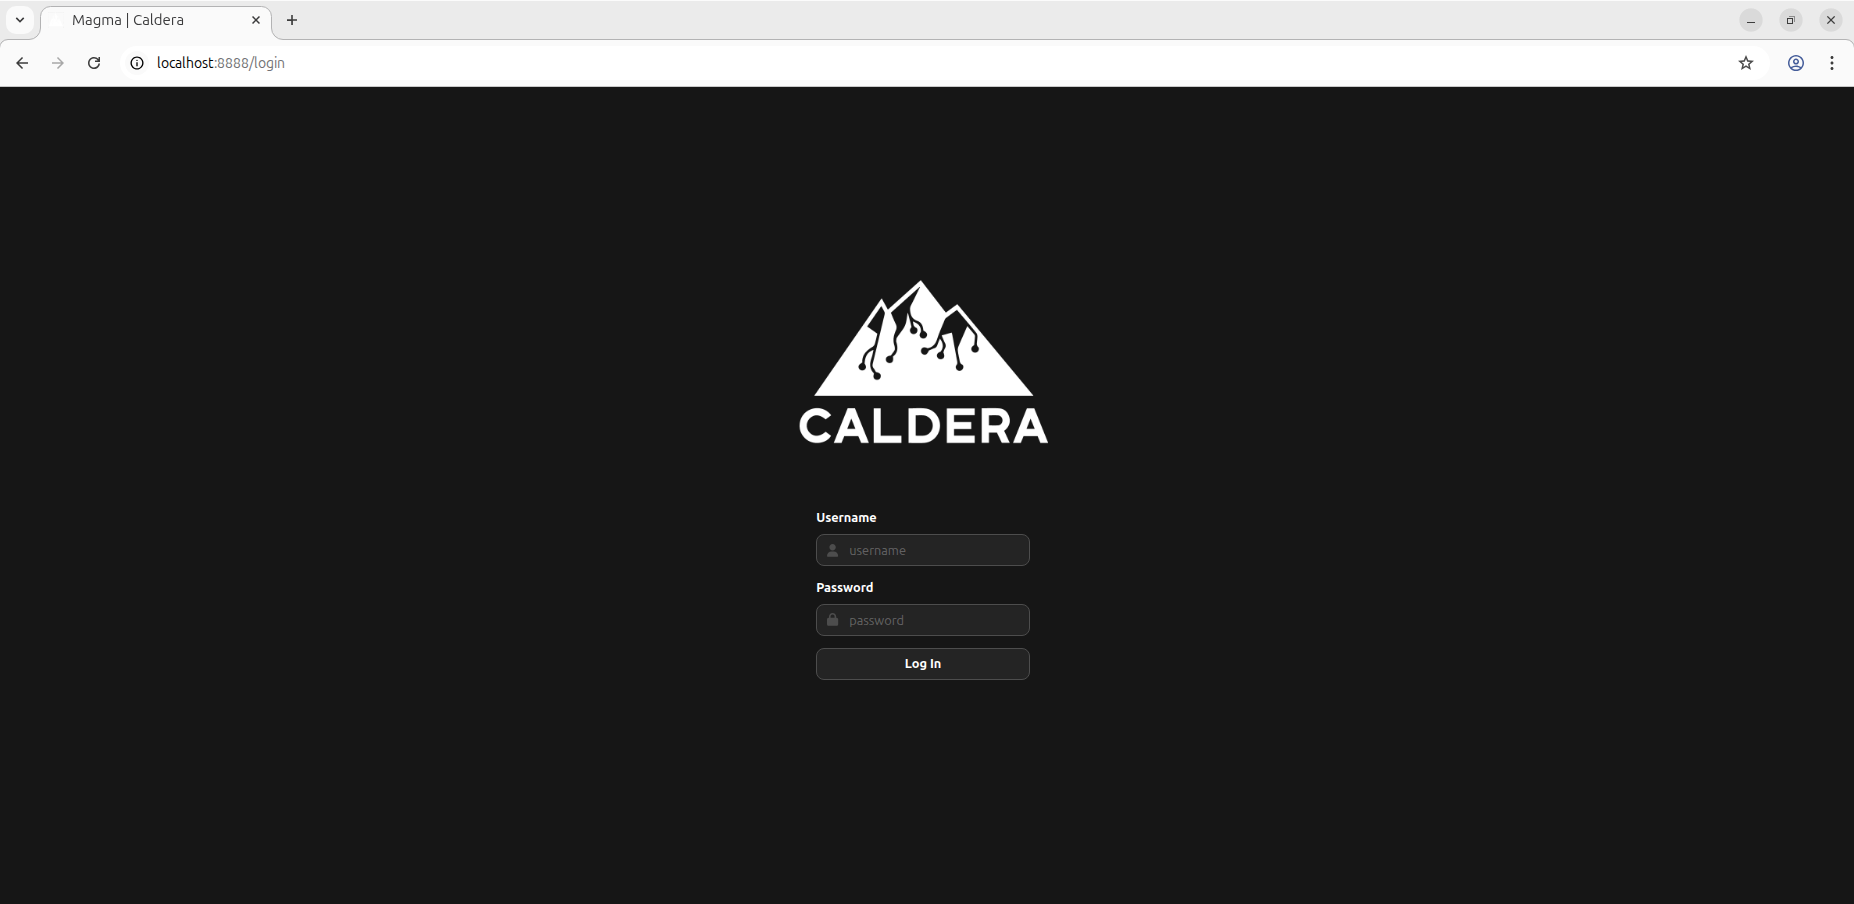
\includegraphics[width=\linewidth]{images/Caldera_login.jpeg}
    \caption{Pagina del login di Caldera}
\end{figure}
\noindent
La schermata seguente rappresenta l'homepage del server. Essa contiene un insieme di resoconti raffigurati mediante dei semplici grafi riguardo gli \textit{agents} inviati, le \textit{operations} create, il numero di \textit{abilities} ed \textit{adversaries} disponibili attualmente, che essi siano predefiniti o creati dall'utente, infine, l'indirizzo IP del server da inserire nella configurazione dell'agente che si vuole installare. Nella barra laterale sinistra sono presenti tutte le funzionalità disponibili durante l'uso del framework: sotto la voce \textit{"campaigns"} abbiamo gli strumenti per coordinare i test sugli hosts target; i \textit{"plugins"} rappresentano le feature aggiuntive, con cui l'utente può cimentarsi, in modo da rendere l'utilizzo più entusiasmante; infine, in \textit{"configuration"} sono presenti le attuali impostazioni avviate nel server.
\begin{figure}[H]
    \centering
    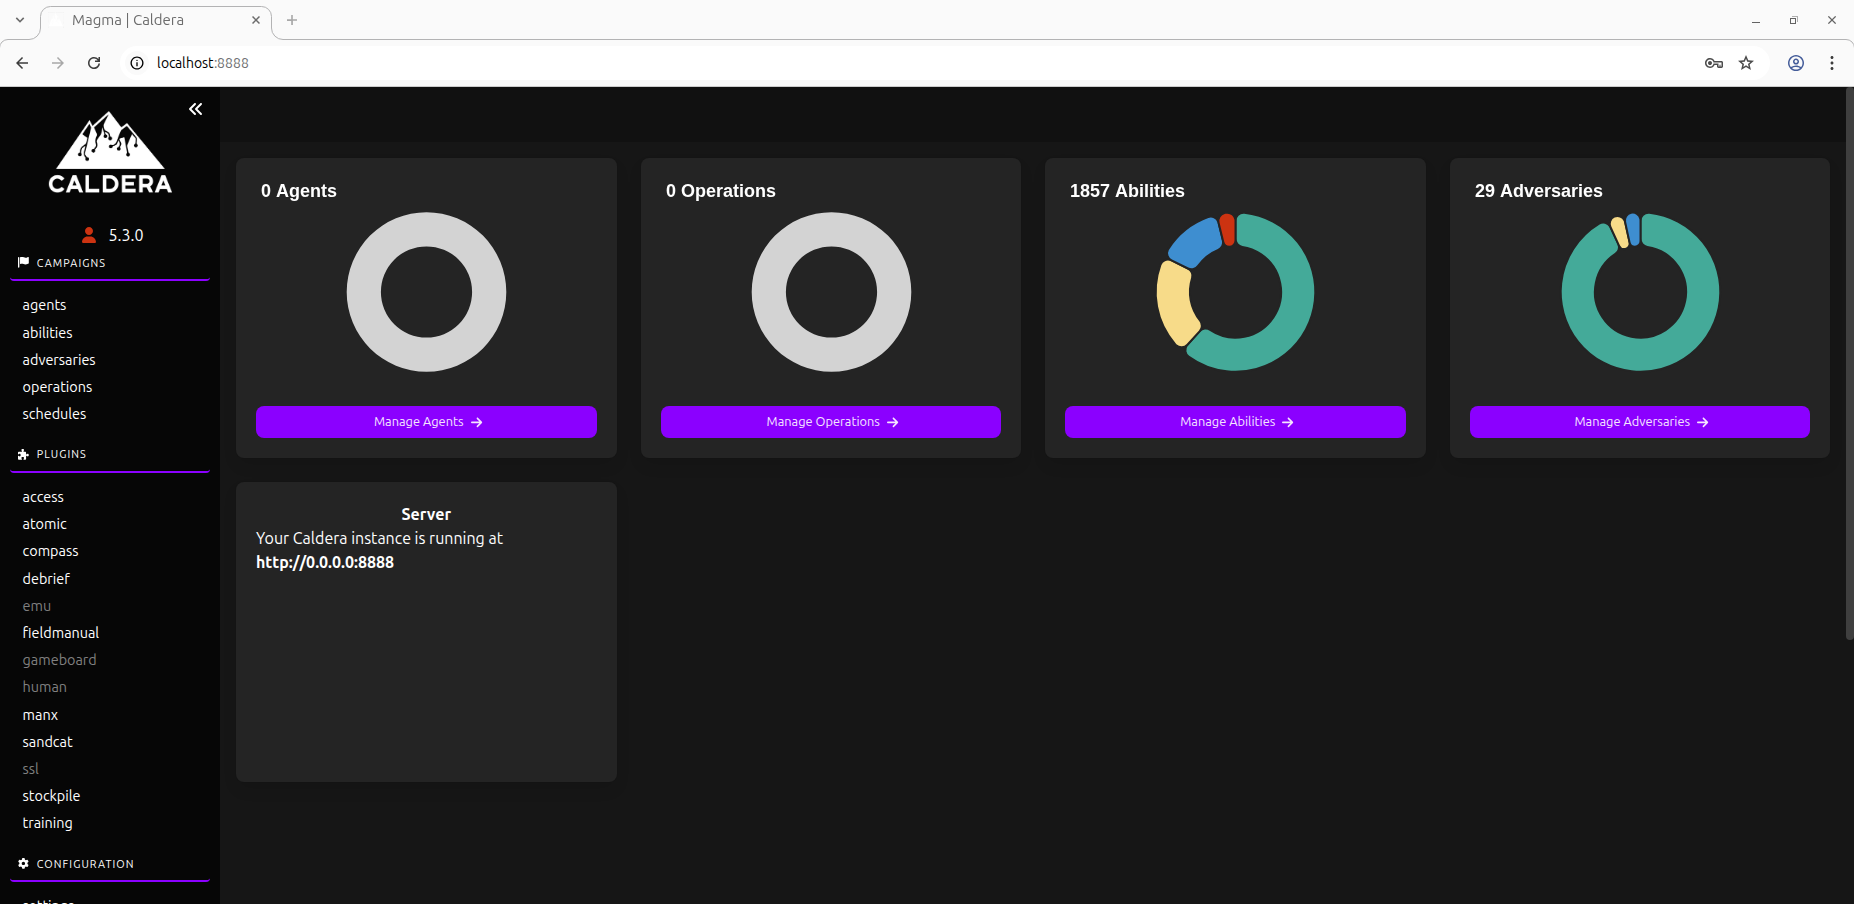
\includegraphics[width=\textwidth]{images/Caldera_home.png}
    \caption{Homepage di Caldera}
\end{figure}
\noindent
Come già spiegato, Caldera comunica come server C2 con dei software collegati in modo da decidere quali \textit{abilities} utilizzare durante le varie operazioni.\\
Una volta selezionato il software da configurare, è possibile decidere il tipo di architettura target e, successivamente, il framework genererà automaticamente degli scripts adatti alla piattaforma selezionata. All'interno della configurazione dell'agente, è possibile cambiare non solo il server con cui creare il contatto HTTP, ma addirittura il nome del processo che questi avrà all'interno del sistema bersaglio; quest'ultima feature permette di rendere la detection del suddetto agente molto più complicata per un membro del Blue Team.\\
\begin{figure}[H]
    \centering
    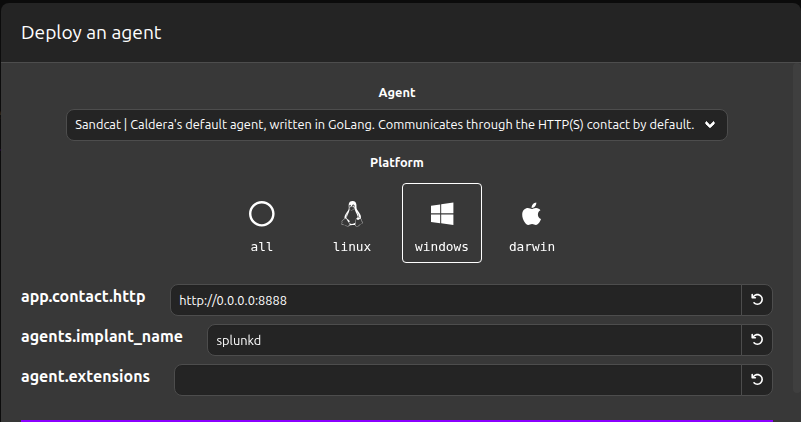
\includegraphics[width=0.7\textwidth, trim={0 1em 0 0}, clip]{images/Caldera_agentSetup.png}
    \caption{Configurazione Sandcat con Caldera}
\end{figure}

\noindent
Oltre allo script generato di default per il software selezionato, Caldera offre la possibilità di scegliere tra diverse variazioni per l'agente in questione. Ne esistono diverse e si invita il lettore ad esplorarle personalmente, di seguito è fornita una lista delle variazioni del software \texttt{Sandcat}.
\begin{itemize}
    \item Un agente distribuito come gruppo Blue Team invece di Red Team.
    \item Un agente compilato con una lista di estensione (richiede GoLang).
    \item Un agente distribuito come P2P con peers incluse durante la compilazione.
\end{itemize}
Una volta che lo script è stato generato, si presenta il problema del come inserirlo all'interno del sistema che si vuole corrompere; questa fase può essere realizzata in diversi modi. Nel caso descritto nelle pagine seguenti è stato fatto uso di una malconfigurazione delle query nel database, sfruttando una tecnica conosciuta come \textsc{SQL Injection}.\\ 
Completate le due fasi sopra descritte, l'agente comparirà nella sezione \textit{Agents} assieme alle sue caratteristiche: nome, PID, tipo di contatto, ecc...\\
\begin{figure}[H]
    \centering
    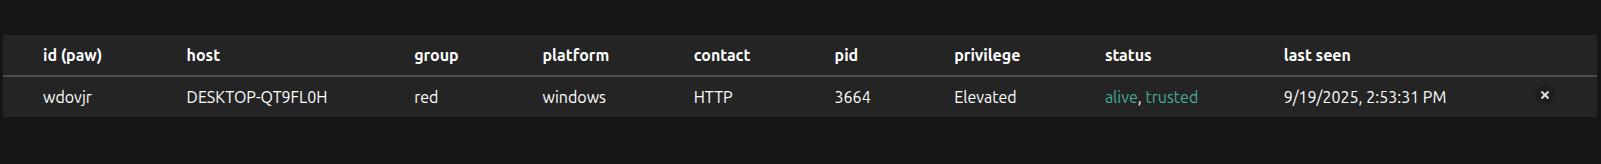
\includegraphics[width=\textwidth]{images/Agent_INS.png}
    \caption{Caratteristiche dell'agente installato}
\end{figure}
\noindent
Da adesso è possibile avviare qualsiasi operazione si voglia, seguendo la serie di possibili profili \textit{Adversaries} offerti da Caldera, oppure creandone uno proprio seguendo i TTPs esplicitati in MITRE ATT\&CK.\\
Nella sezione \textit{Operations} del menù di Caldera, si ha la possibilità di creare ed avviare un'operazione di Red Teaming. Una volta preparata un \textit{operation} e selezionato l'avversario, nella schermata si potrà seguire l'esecuzione di ogni \textit{ability}. Per ogni step è possibile visualizzare una miniatura in cui sono raffigurati i comandi eseguiti, relativo output ed uno stato variabile tra:
    \begin{itemize}
        \item \textcolor{yellow}{Giallo}: L'attività corrente e in fase di esecuzione nel target.
        \item \textcolor{green}{Verde}: L'agente è riuscito a concludere l'\textit{ability} senza imprevisti.
        \item \textcolor{red}{Rosso}: L'attività non è andata a buon fine per qualche motivo (visionare l'output generato). 
        \item \textcolor{cyan}{Blu-verde}: È stato raggiunto il timeout per l'\textit{ability}.
    \end{itemize}
L'output può contenere un informazione (\textit{fact}) fondamentale al fine di continuare le \textit{abilities} successive. Per questo motivo, è importante selezionare con cura e sistematicamente l'ordine con cui andare ad eseguire ogni azione.
\begin{figure}[H]
    \centering
    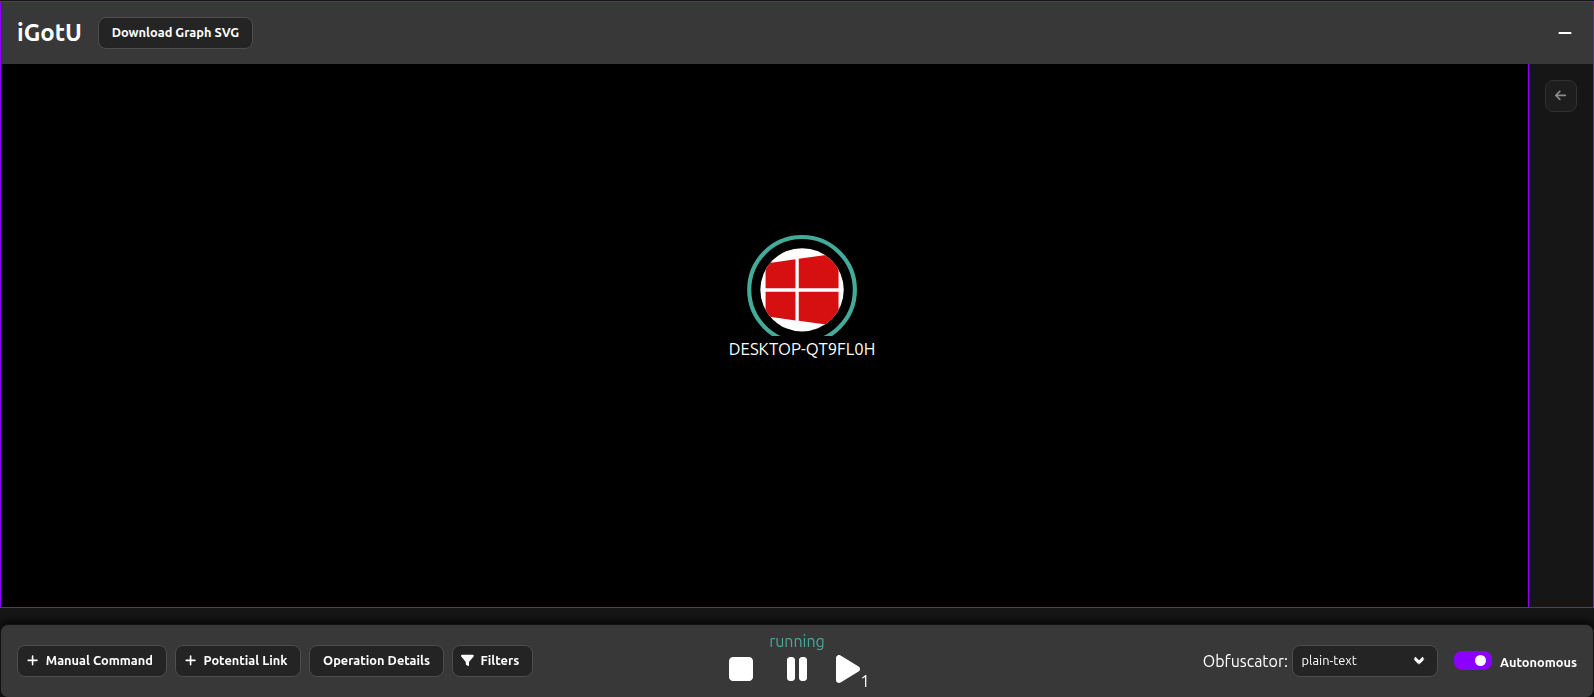
\includegraphics[width=\textwidth]{images/Caldera_Operation.png}
    \caption{Esempio di grafo di una operazione Caldera}
\end{figure}
Come si può notare dall'immagine, l'utente può decidere se stoppare in anticipo l'operazione o, semplicemente, metterla in pausa a causa di problemi che possono verificarsi. Inoltre, se si sta lavorando in uno scenario avente un numero considerevole di sistemi interconnessi sotto la stessa rete, il grafo raffigurato ha la possibilità di espandersi; in questo modo, si ha una visione completa degli agenti operativi.\\ 
Una volta scanditi tutti gli stadi dell'\textit{operation}, verrà generato un resoconto, contenente i log di ogni evento, da poter scaricare ed offrire agli amministratori della sicurezza dell'azienda.